%%%%%%%%%%%%%%%%%%%%%%%%%%%%%%%%%%%%%%%%%%%%%%%%%%%%%%%%%%%%%%%%%%%%%%%%%%
\section{Colors}
%%%%%%%%%%%%%%%%%%%%%%%%%%%%%%%%%%%%%%%%%%%%%%%%%%%%%%%%%%%%%%%%%%%%%%%%%%
%
%%%%%%%%%%%%%%%%%%%%%%%%%%%%%%%%%%%%%%%%%%%%%%%%%%%%%%%%%%%%%%%%%%%%%%%%%%
\subsection*{Vocabulary}
%%%%%%%%%%%%%%%%%%%%%%%%%%%%%%%%%%%%%%%%%%%%%%%%%%%%%%%%%%%%%%%%%%%%%%%%%%
%
\begin{supertabular}{p{2,5cm}|ll}
    %
    \index{jelo}
    \textbf{\dots jelo}        &  & \textit{adjective}: yellowish, yellowy                                \\ % no-dictionary
    \textbf{jelo}              &  & \textit{noun}: yellow, light green                                    \\ % no-dictionary
                               &  &                                                                       \\ % no-dictionary
    %
    \index{kule}
    \textbf{\dots kule}        &  & \textit{adjective}: colourful, pigmented, painted                     \\ % no-dictionary
    \textbf{kule}              &  & \textit{noun}: color, colour, paint, ink, dye, hue                    \\ % no-dictionary
    \textbf{kule (e \dots)}    &  & \textit{verb transitive}: to paint, to color                          \\ % no-dictionary
                               &  &                                                                       \\ % no-dictionary
    %
    \index{laso}
    \textbf{\dots laso}        &  & \textit{adjective}: bluish, bluey                                     \\ % no-dictionary
    \textbf{laso}              &  & \textit{noun}: blue, blue-green                                       \\ % no-dictionary
                               &  &                                                                       \\ % no-dictionary
    %
    \index{loje}
    \textbf{\dots loje}        &  & \textit{adjective}: reddish, ruddy, pink, pinkish, gingery            \\ % no-dictionary
    \textbf{loje}              &  & \textit{noun}: red                                                    \\ % no-dictionary
                               &  &                                                                       \\ % no-dictionary
    %
    \index{pimeja}
    \textbf{\dots pimeja}      &  & \textit{adjective}: black, dark                                       \\ % no-dictionary
    \textbf{pimeja}            &  & \textit{noun}: darkness, shadows                                      \\ % no-dictionary
    \textbf{pimeja (e \dots)}  &  & \textit{verb transitive}: to darken                                   \\ % no-dictionary
                               &  &                                                                       \\ % no-dictionary
    %
    \index{sitelen}
    \textbf{\dots sitelen}     &  & \textit{adjective}: figurative, pictorial, metaphorical, metaphorisch \\ % no-dictionary
    \textbf{\dots sitelen}     &  & \textit{adverb}: pictorially                                          \\ % no-dictionary
    \textbf{sitelen}           &  & \textit{noun}: picture, image, representation, symbol, mark, writing  \\ % no-dictionary
    \textbf{sitelen (e \dots)} &  & \textit{verb transitive}: to draw, to write                           \\ % no-dictionary
                               &  &                                                                       \\ % no-dictionary
    %
    \index{walo}
    \textbf{\dots walo}        &  & \textit{adjective}: white, whitish, light-coloured, pale              \\ % no-dictionary
    \textbf{walo}              &  & \textit{noun}: white thing or part, whiteness, lightness              \\ % no-dictionary
    \textbf{walo (e \dots)}    &  & \textit{verb transitive}: to whiten, to whitewash                     \\ % no-dictionary
    %
\end{supertabular} \\
%
%
%%%%%%%%%%%%%%%%%%%%%%%%%%%%%%%%%%%%%%%%%%%%%%%%%%%%%%%%%%%%%%%%%%%%%%%%%%
\newpage
%
\subsection*{Color Combinations}
\subsubsection*{A Shade of Colour}
%
\index{color}
%%%%%%%%%%%%%%%%%%%%%%%%%%%%%%%%%%%%%%%%%%%%%%%%%%%%%%%%%%%%%%%%%%%%%%%%%%
%
In Toki Pona there are no words for the colors purple, green, grey, etc.
But you can create colors from several words.
One uses one of these nouns \textit{jelo}, \textit{laso}, \textit{loje}, \textit{pimeja} or \textit{walo}.
Then use these adjectives \textit{jelo}, \textit{laso}, \textit{loje}, \textit{pimeja}, or \textit{walo}.

\begin{supertabular}{p{5,5cm}|ll}
    laso loje li ' pona, tawa mi.   &  & Purple (reddish blue) is my favourite colour.  \\
    laso jelo li ' pona, tawa mi.   &  & Green (yellowish blue) is my favourite colour. \\
    loje jelo li ' pona, tawa mi.   &  & Orange (yellowish red) is my favourite colour. \\
    loje walo li ' pona, tawa mi.   &  & Pink (whitish red) is my favourite colour.     \\
    walo pimeja li ' pona, tawa mi. &  & Grey (dark white) is my favourite colour.      \\
\end{supertabular}

It is also possible to form colors from a noun and several adjectives.
The goal of Toki Pona is however the simplicity.
Therefore, avoid complex word compositions.
% Incidentally, the order of the colours doesn't matter.

\begin{supertabular}{p{5,5cm}|ll}
    laso loje  li ' pona, tawa mi. &  & Purple is my favourite colour. \\ % no-dictionary
    loje laso  li ' pona, tawa mi. &  & Purple is my favourite colour. \\
\end{supertabular}

Colors are usually used as adjectives because they describe nouns.
The adjectives \textit{loje} and \textit{laso} describe the noun \textit{len} here.

\begin{supertabular}{p{5,5cm}|ll}
    len loje laso mi li ' pona, tawa mi. &  & I like this purple t-shirt. \\
\end{supertabular}

%
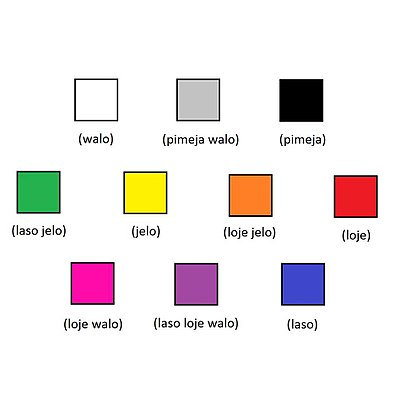
\includegraphics[scale=0.4]{colors.png}
%
%%%%%%%%%%%%%%%%%%%%%%%%%%%%%%%%%%%%%%%%%%%%%%%%%%%%%%%%%%%%%%%%%%%%%%%%%%
\subsubsection*{Samples in Several Shades of Colour}
%
%%%%%%%%%%%%%%%%%%%%%%%%%%%%%%%%%%%%%%%%%%%%%%%%%%%%%%%%%%%%%%%%%%%%%%%%%%
%
Suppose that you have a shirt that have pattern with different colors (red and blue).
However, you can't call it \textit{len loje laso}, because that means 'purple shirt'.
The colours must be separated grammatically.
Each color of the pattern is described with a noun and optional adjectives.
To separate these color nouns with their adjectives we use the conjunction \textit{en}.
To separate the patterned item from its colours the separator serves \textit{pi}.
\textit{len}, \textit{loje} and \textit{laso} are nouns here.

\begin{supertabular}{p{5,5cm}|ll}
    len ni pi loje en laso li ' pona, tawa mi.                             &  & I like this red and blue patterned t-shirt.                    \\
    tomo pi jelo en loje pi meli Susan en mije jan Ken li ' nasa, tawa mi. &  & Susan and Ken's yellow and blue patterned house looks strange. \\
\end{supertabular}

%
%%%%%%%%%%%%%%%%%%%%%%%%%%%%%%%%%%%%%%%%%%%%%%%%%%%%%%%%%%%%%%%%%%%%%%%%%%
\subsection*{The Noun \textit{kule}}
%
\index{\textit{kule}!noun}
%%%%%%%%%%%%%%%%%%%%%%%%%%%%%%%%%%%%%%%%%%%%%%%%%%%%%%%%%%%%%%%%%%%%%%%%%%
%
The noun \textit{kule} means 'color'.

\begin{supertabular}{p{5,5cm}|ll}
    ni li ' kule seme? &  & What color is that? \\
\end{supertabular}

%
%%%%%%%%%%%%%%%%%%%%%%%%%%%%%%%%%%%%%%%%%%%%%%%%%%%%%%%%%%%%%%%%%%%%%%%%%%
\subsection*{The Adjective \textit{kule}}
%
\index{\textit{kule}!adjective}
%%%%%%%%%%%%%%%%%%%%%%%%%%%%%%%%%%%%%%%%%%%%%%%%%%%%%%%%%%%%%%%%%%%%%%%%%%
%
The adjective \textit{kule} means 'colourful', 'pigmented' or 'painted'.

\begin{supertabular}{p{5,5cm}|ll}
    len kule li ' pona, tawa mi. &  & I like the colourful dress. \\
\end{supertabular}

%
%%%%%%%%%%%%%%%%%%%%%%%%%%%%%%%%%%%%%%%%%%%%%%%%%%%%%%%%%%%%%%%%%%%%%%%%%%
\subsection*{The Transitive Verb \textit{kule}}
%
\index{\textit{kule}!verb}
%%%%%%%%%%%%%%%%%%%%%%%%%%%%%%%%%%%%%%%%%%%%%%%%%%%%%%%%%%%%%%%%%%%%%%%%%%
%
The transitive verb \textit{kule} means 'to dye'.

\begin{supertabular}{p{5,5cm}|ll}
    ona li kule ala kule e len? &  & Does she dye the dress? \\
    mi kule e lipu              &  & I dye the dress.        \\
\end{supertabular}

%
%%%%%%%%%%%%%%%%%%%%%%%%%%%%%%%%%%%%%%%%%%%%%%%%%%%%%%%%%%%%%%%%%%%%%%%%%%
\subsection*{The Noun \textit{sitelen}}
%
\index{\textit{sitelen}!noun}
%%%%%%%%%%%%%%%%%%%%%%%%%%%%%%%%%%%%%%%%%%%%%%%%%%%%%%%%%%%%%%%%%%%%%%%%%%
%
The noun \textit{sitelen} means 'picture' or 'image'.

\begin{supertabular}{p{5,5cm}|ll}
    sitelen tawa                                      &  & movie, TV show                                  \\
    sitelen tawa 'Fahrenheit 9/11' li pona, tawa mi.  &  & I like the movie 'Fahrenheit 9/11'.             \\
    sitelen tawa 'Bowling for Columbine' li pona kin. &  & The movie 'Bowling for Columbine' is also good. \\
    sitelen ma                                        &  & map                                             \\
    o pana e sitelen ma, tawa mi.                     &  & Give me the map.                                \\
\end{supertabular}

%
%%%%%%%%%%%%%%%%%%%%%%%%%%%%%%%%%%%%%%%%%%%%%%%%%%%%%%%%%%%%%%%%%%%%%%%%%%
\subsection*{The Adjective \textit{sitelen}}
%
\index{\textit{sitelen}!adjective}
%%%%%%%%%%%%%%%%%%%%%%%%%%%%%%%%%%%%%%%%%%%%%%%%%%%%%%%%%%%%%%%%%%%%%%%%%%
%
The adjective \textit{sitelen} means 'figurative', 'pictorial', 'metaphorical' or 'metaphorisch' or 'writen down'.

\begin{supertabular}{p{5,5cm}|ll}
    toki sitelen li ' pona, tawa jan ali. &  & Written language (writing) is good for all people. \\
\end{supertabular}

%
%%%%%%%%%%%%%%%%%%%%%%%%%%%%%%%%%%%%%%%%%%%%%%%%%%%%%%%%%%%%%%%%%%%%%%%%%%
\subsection*{The Transitive Verb \textit{sitelen}}
%
\index{\textit{sitelen}!verb}
%%%%%%%%%%%%%%%%%%%%%%%%%%%%%%%%%%%%%%%%%%%%%%%%%%%%%%%%%%%%%%%%%%%%%%%%%%
%
The transitive verb \textit{sitelen} means to 'draw' or to 'write'.

\begin{supertabular}{p{5,5cm}|ll}
    ona li sitelen ala sitelen?     &  & Does he draw?                \\
    mi sitelen e sitelen, lon lipu. &  & I draw the picture on paper. \\
\end{supertabular}

%
%%%%%%%%%%%%%%%%%%%%%%%%%%%%%%%%%%%%%%%%%%%%%%%%%%%%%%%%%%%%%%%%%%%%%%%%%%
\subsection*{The Adverb \textit{sitelen}}
%
\index{\textit{sitelen}!adverb}
%%%%%%%%%%%%%%%%%%%%%%%%%%%%%%%%%%%%%%%%%%%%%%%%%%%%%%%%%%%%%%%%%%%%%%%%%%
%
The adverb \textit{sitelen} means 'pictorially'.

\begin{supertabular}{p{5,5cm}|ll}
    ona li toki sitelen e ni. &  & She says this very figuratively. \\
\end{supertabular}

%
%%%%%%%%%%%%%%%%%%%%%%%%%%%%%%%%%%%%%%%%%%%%%%%%%%%%%%%%%%%%%%%%%%%%%%%%%%
\newpage
%
\subsection*{Practice (Answers: Page~\pageref{'colors'})}
%%%%%%%%%%%%%%%%%%%%%%%%%%%%%%%%%%%%%%%%%%%%%%%%%%%%%%%%%%%%%%%%%%%%%%%%%%
%
Please write down your answers and check them afterwards.

\begin{supertabular}{p{5,5cm}|ll}
    Which kinds of word are possible in the slot after the conjunction \textit{en}? &  & \\ % no-dictionary
    How are color pattern of an item described in \textit{toki pona}?               &  & \\ % no-dictionary
    How are color tones described for which there is no word in \textit{toki pona}? &  & \\ % no-dictionary
    Which kinds of word are possible in the slot after the separator \textit{pi}?   &  & \\ % no-dictionary
    What kinds of words have the words for colors in \textit{toki pona}?            &  & \\ % no-dictionary
\end{supertabular}

Try to translate these sentences.
You can use the tool \textit{Toki Pona Parser} (\cite{www:rowa:02}) for spelling and grammar check.

\begin{supertabular}{p{5,5cm}|ll}
    I don't see the blue bag.                &  & \\ % no-dictionary
    A little green person came from the sky. &  & \\ % no-dictionary
    I like the color purple.                 &  & \\ % no-dictionary
    The sky is blue.                         &  & \\ % no-dictionary
    Look at that red bug.                    &  & \\ % no-dictionary
    I want the map.                          &  & \\ % no-dictionary
    Do you watch The X-Files?                &  & \\  % no-dictionary
    Which color do you like?*                &  & \\  % no-dictionary
    Is it red?                               &  & \\ % no-dictionary
\end{supertabular}

\begin{supertabular}{p{5,5cm}|ll}
    ni li pimeja ala pimeja e suno?                      &  & \\ % no-dictionary
    suno li ' jelo.                                      &  & \\ % no-dictionary
    telo suli li ' laso.                                 &  & \\ % no-dictionary
    mi wile moku e kili loje.                            &  & \\ % no-dictionary
    ona li kule e tomo tawa.                             &  & \\ % no-dictionary
    len pi loje en laso pi meli sina li ' pona, tawa mi. &  & \\ % no-dictionary
\end{supertabular}

* Think: 'Which color is good for you?'

And now try reading this Toki Pona poem.

\begin{supertabular}{p{5,5cm}|ll}
    ma mi li ' pimeja. &  & \\ % no-dictionary
    kalama ala li lon  &  & \\ % no-dictionary
    mi lape. mi sona.  &  & \\ % no-dictionary
\end{supertabular}
%%%%%%%%%%%%%%%%%%%%%%%%%%%%%%%%%%%%%%%%%%%%%%%%%%%%%%%%%%%%%%%%%%%%%%%%%%
% eof
